\section{Силовые полупроводниковые приборы}
Должны знать на уровне пользователя.

Первым прибором был электровакуумный (кенотрон).

% http://tex.stackexchange.com/questions/66216/draw-arc-in-tikz-when-center-of-circle-is-specified
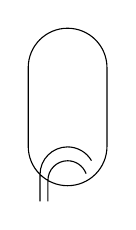
\begin{tikzpicture}
\draw(0,1)--(0,2)arc(180:0:0.5)--(1,1)arc(0:-180:0.5)

%(0.3,0.5)--(0.3,{1-sqrt(0.5-0.2*0.2)})arc(180:20:0.2)
(0.25,0.3)--(0.25,{1-sqrt(0.5*0.5-0.25*0.25)})arc(180:20:0.25)
(0.15,0.3)--(0.15,{1-sqrt(0.5*0.5-0.35*0.35)})arc(180:30:0.35)
;
\end{tikzpicture}
Катод с помощью термоэлектронной эмиссии испускает электроны.
